\documentclass[a4paper, 12pt, finnish]{report}
\usepackage[utf8]{inputenc}
\usepackage{amsfonts}
\usepackage{graphics}
\usepackage[finnish]{babel}
\usepackage{titlesec}
\titleformat{\chapter}
{\Large\bfseries}
{}            
{0pt}      
{\huge} 

\newcommand{\topic}{Hakemukseni AYYn hallitukseen kaudelle 2017}
\usepackage{hyperref}
\hypersetup{pdfpagemode=UseNone, pdfstartview=FitH, colorlinks=true,urlcolor=red,linkcolor=blue,citecolor=black,pdftitle={\topic},pdfauthor={Onni Lampi}}
\setlength{\parindent}{0mm}
\setlength{\emergencystretch}{15pt}
\newcommand*{\findate}{\the\day.\the\month.\the\year}

\begin{document}



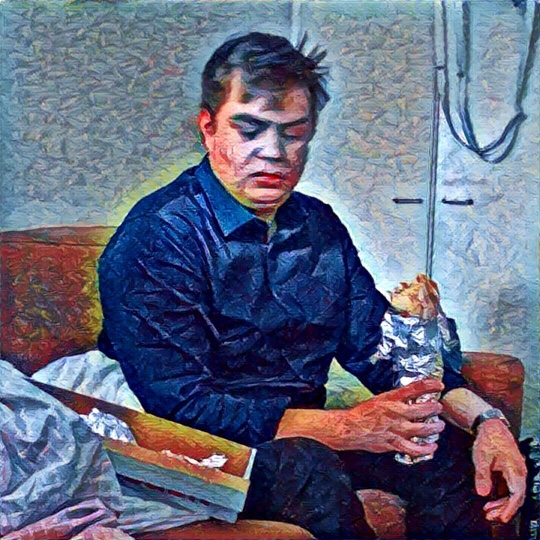
\includegraphics{Onni.jpg}
\section*{\topic}
Olen 24-vuotias 4. vuoden tietoliikennetekniikan opiskelija.
Olen kotoisin Helsingistä ja tässä muutaman opiskeluvuoden aikana AYY on tullut minulle hyvin läheiseksi ja rakkaaksi organisaatioksi.\\

Olen toiminut erinäisissä vapaaehtoishommissa ylioppilaskunnassa käytännössä koko opiskeluaikani.
Näihin kuuluu mm. vastuut killan ISOvastaavana, ammattiainekerhon puheenjohtajana ja edustajistossa toimiminen ryhmäpuheenjohtajan asemassa.


\section*{Yhteystiedot}
Onni Lampi\\
040 702 3841\\
omnez@IRCnet, telegram\\
contact@onnilampi.fi
\end{document}
